%!Mode:: "TeX:UTF-8"
\documentclass[a4paper,11pt,UTF8]{ctexart}

\usepackage{indentfirst} %缩进
\usepackage{xeCJK}    %使用系统字体
\usepackage{fancyhdr} %自定义页眉页脚
\pagestyle{empty}                   %不设置页眉页脚
\usepackage{amsmath, amsthm, amssymb, amsfonts} %数学公式
\usepackage[a4paper,left=3cm,right=3cm,top=3cm,bottom=3cm]{geometry}
%\usepackage[tmargin=1in,bmargin=1in,lmargin=1.25in,rmargin=1.25in]{geometry}.
\usepackage{booktabs} %插入表格
\usepackage[section]{placeins} %避免浮动
\usepackage{listings} %插入代码
\usepackage{ctex}     %中文宏包
\usepackage[svgnames, table]{xcolor} %彩色表格
\usepackage{algorithm}          %伪代码
\usepackage{algorithmicx}
\usepackage{algpseudocode}
\usepackage{algorithm,algpseudocode,float}
\usepackage{lipsum}
\usepackage{enumitem}           %调整列举环境
\usepackage{url}
\usepackage{fontspec,xunicode}
\defaultfontfeatures{Mapping=tex-text} %如果没有它,会有一些 tex 特殊字符无法正常使用,比如连字符。
\usepackage{wrapfig}
\usepackage{graphicx}
\graphicspath{{imgs/}}

%%%%%%%%%%%%%%%%%%%%%%%%%%%%%%%%%%%%%%%%%%%%%%%%%%%%%%%%%%%%%%%%
% 缩进及行间距
%%%%%%%%%%%%%%%%%%%%%%%%%%%%%%%%%%%%%%%%%%%%%%%%%%%%%%%%%%%%%%%%
\setlength{\parindent}{22pt} %重新定义缩进长度
\setlength{\baselineskip}{20pt}  %定义行间距
%\renewcommand{\baselinestretch}{1.1} %定义行间距
%%%%%%%%%%%%%%%%%%%%%%%%%%%%%%%%%%%%%%%%%%%%%%%%%%%%%%%%%%%%%%%%
% 数学符号
%%%%%%%%%%%%%%%%%%%%%%%%%%%%%%%%%%%%%%%%%%%%%%%%%%%%%%%%%%%%%%%%
\newcommand\pd{\partial}
\newcommand\dd{\thinspace\mathrm{d}}
\newcommand\pdone[2]{\frac{\pd #1}{\pd #2}}
\newcommand\pdtwo[2]{\frac{\pd^2 #1}{\pd #2 ^2}}
\newcommand\ddone[2]{\frac{\dd #1}{\dd #2}}
\newcommand\ddtwo[2]{\frac{\dd^2 #1}{\dd #2 ^2}}
%%%%%%%%%%%%%%%%%%%%%%%%%%%%%%%%%%%%%%%%%%%%%%%%%%%%%%%%%%%%%%%%
% 列表设置
%%%%%%%%%%%%%%%%%%%%%%%%%%%%%%%%%%%%%%%%%%%%%%%%%%%%%%%%%%%%%%%%
\setenumerate{fullwidth,itemindent=\parindent,listparindent=\parindent,itemsep=0ex,partopsep=0pt,parsep=0ex}
\setenumerate[2]{label=\alph*),leftmargin=1.5em}  %二级item设置
\setitemize{itemindent=38pt,leftmargin=0pt,itemsep=-0.4ex,listparindent=26pt,partopsep=0pt,parsep=0.5ex,topsep=-0.25ex}
\setdescription{itemindent=38pt,leftmargin=0pt,itemsep=-0.4ex,listparindent=26pt,partopsep=0pt,parsep=0.5ex,topsep=-0.25ex}

%%%%%%%%%%%%%%%%%%%%%%%%%%%%%%%%%%%%%%%%%%%%%%%%%%%%%%%%%%%%%%%%
% 图的标题行间距设置
%%%%%%%%%%%%%%%%%%%%%%%%%%%%%%%%%%%%%%%%%%%%%%%%%%%%%%%%%%%%%%%%
\newcommand{\bottomcaption}{%
\setlength{\abovecaptionskip}{6pt}%
\setlength{\belowcaptionskip}{6pt}%
\caption}


%%%%%%%%%%%%%%%%%%%%%%%%%%%%%%%%%%%%%%%%%%%%%%%%%%%%%%%%%%%%%%%%
% 字体定义
%%%%%%%%%%%%%%%%%%%%%%%%%%%%%%%%%%%%%%%%%%%%%%%%%%%%%%%%%%%%%%%%
\setmainfont{Times New Roman}  %默认英文字体.serif是有衬线字体sans serif无衬线字体
\setmonofont{Consolas}
\setCJKmainfont[ItalicFont={楷体}, BoldFont={黑体}]{宋体}%衬线字体 缺省中文字体为
\setCJKsansfont{黑体}
\punctstyle{hangmobanjiao}
%-----------------------xeCJK下设置中文字体------------------------------%
\setCJKfamilyfont{song}{SimSun}                             %宋体 song
\newcommand{\song}{\CJKfamily{song}}
\setCJKfamilyfont{fs}{FangSong}                      %仿宋  fs
\newcommand{\fs}{\CJKfamily{fs}}
\setCJKfamilyfont{ktgb}{KaiTi}                      %楷体2312 ktgb
\newcommand{\ktgb}{\CJKfamily{ktgb}}
\setCJKfamilyfont{yh}{Microsoft YaHei}                    %微软雅黑 yh
\newcommand{\yh}{\CJKfamily{yh}}
\setCJKfamilyfont{hei}{SimHei}                              %黑体  hei
\newcommand{\hei}{\CJKfamily{hei}}
\setCJKfamilyfont{hwxk}{STXingkai}                                %华文行楷  hwxk
\newcommand{\hwxk}{\CJKfamily{hwxk}}
%------------------------------设置字体大小------------------------%
\newcommand{\shiyanbaogao}{\fontsize{36pt}{\baselineskip}\selectfont}
\newcommand{\chuhao}{\fontsize{42pt}{\baselineskip}\selectfont}     %初号
\newcommand{\xiaochuhao}{\fontsize{36pt}{\baselineskip}\selectfont} %小初号
\newcommand{\yihao}{\fontsize{28pt}{\baselineskip}\selectfont}      %一号
\newcommand{\erhao}{\fontsize{21pt}{\baselineskip}\selectfont}      %二号
\newcommand{\xiaoerhao}{\fontsize{18pt}{\baselineskip}\selectfont}  %小二号
\newcommand{\sanhao}{\fontsize{15.75pt}{\baselineskip}\selectfont}  %三号
\newcommand{\sihao}{\fontsize{14pt}{\baselineskip}\selectfont}       %四号
\newcommand{\xiaosihao}{\fontsize{12pt}{\baselineskip}\selectfont}  %小四号
\newcommand{\wuhao}{\fontsize{10.5pt}{\baselineskip}\selectfont}    %五号
\newcommand{\xiaowuhao}{\fontsize{9pt}{\baselineskip}\selectfont}   %小五号
\newcommand{\liuhao}{\fontsize{7.875pt}{\baselineskip}\selectfont}  %六号
\newcommand{\qihao}{\fontsize{5.25pt}{\baselineskip}\selectfont}    %七号

%%%%%%%%%%%%%%%%%%%%%%%%%%%%%%%%%%%%%%%%%%%%%%%%%%%%%%%%%%%%%%%%
% 图题字体大小相同
%%%%%%%%%%%%%%%%%%%%%%%%%%%%%%%%%%%%%%%%%%%%%%%%%%%%%%%%%%%%%%%%
\usepackage{caption}
\captionsetup{font={footnotesize}}   % footnotesize = 9pt
\captionsetup[lstlisting]{font={footnotesize}}

%%%%%%%%%%%%%%%%%%%%%%%%%%%%%%%%%%%%%%%%%%%%%%%%%%%%%%%%%%%%%%%%
% 重定义枚举编号为 1),2)...
%%%%%%%%%%%%%%%%%%%%%%%%%%%%%%%%%%%%%%%%%%%%%%%%%%%%%%%%%%%%%%%%
\renewcommand{\labelenumi}{\theenumi)}

%%%%%%%%%%%%%%%%%%%%%%%%%%%%%%%%%%%%%%%%%%%%%%%%%%%%%%%%%%%%%%%%
% 标题名称中文化
%%%%%%%%%%%%%%%%%%%%%%%%%%%%%%%%%%%%%%%%%%%%%%%%%%%%%%%%%%%%%%%%
\renewcommand\figurename{\hei 图}
\renewcommand\tablename{\hei 表}
\renewcommand\lstlistingname{\hei 代码}
\renewcommand{\algorithmicrequire}{\textbf{输入:}}
\renewcommand{\algorithmicensure}{\textbf{输出:}}
\newtheorem{define}{定义}

%%%%%%%%%%%%%%%%%%%%%%%%%%%%%%%%%%%%%%%%%%%%%%%%%%%%%%%%%%%%%%%%
% 代码设置
%%%%%%%%%%%%%%%%%%%%%%%%%%%%%%%%%%%%%%%%%%%%%%%%%%%%%%%%%%%%%%%%
\lstset{
 columns=fixed,
 numbers=left,                                        % 在左侧显示行号
 numberstyle=\tiny\color{gray},                       % 设定行号格式
 frame=single,                                        % 单线背景边框
 breaklines=true,                                     % 设定LaTeX对过长的代码行进行自动换行
 keywordstyle=\color[RGB]{40,40,255},                 % 设定关键字颜色
 numberstyle=\footnotesize\color{darkgray},
 commentstyle=\it\color[RGB]{0,96,96},                % 设置代码注释的格式
 stringstyle=\rmfamily\slshape\color[RGB]{128,0,0},   % 设置字符串格式
 showstringspaces=false,                              % 不显示字符串中的空格
 language=java,                                        % 设置语言
 basicstyle=\linespread{1.0}\xiaowuhao\ttfamily,                      % 字体字号
 %lineskip=10pt,
 %baselinestretch=1,
}

%%%%%%%%%%%%%%%%%%%%%%%%%%%%%%%%%%%%%%%%%%%%%%%%%%%%%%%%%%%%%%%%
% 伪代码分页
%%%%%%%%%%%%%%%%%%%%%%%%%%%%%%%%%%%%%%%%%%%%%%%%%%%%%%%%%%%%%%%%
\makeatletter
\renewcommand{\ALG@name}{算法}
\newenvironment{breakablealgorithm}
  {% \begin{breakablealgorithm}
   \begin{center}
     \refstepcounter{algorithm}% New algorithm
     \hrule height.8pt depth0pt \kern2pt% \@fs@pre for \@fs@ruled
     \renewcommand{\caption}[2][\relax]{% Make a new \caption
       {\raggedright\textbf{\ALG@name~\thealgorithm} ##2\par}%
       \ifx\relax##1\relax % #1 is \relax
         \addcontentsline{loa}{algorithm}{\protect\numberline{\thealgorithm}##2}%
       \else % #1 is not \relax
         \addcontentsline{loa}{algorithm}{\protect\numberline{\thealgorithm}##1}%
       \fi
       \kern2pt\hrule\kern2pt
     }
  }{% \end{breakablealgorithm}
     \kern2pt\hrule\relax% \@fs@post for \@fs@ruled
   \end{center}
  }
\makeatother

\title{一阶电路的研究}
\author{PB19000132 苗立扬  PB18020556 戴佳乐}


%\institute{中国科学技术大学}

% =============================================
% Part 1 Edit the info
% =============================================



\newcommand{\course}{电子线路实验(1)}
\newcommand{\newtitle}{一阶电路的研究}

% =============================================
% Part 1 Main document
% =============================================
\begin{document}
\maketitle

% =============================================
% Part 2 Main document
% =============================================

\section{实验目的}
1. 了解 $\mathrm{RC}$ 正弦波振荡器的组成


2. 理解振荡器的起振条件和平衡条件


3. 掌握 $\mathbf{R C}$ 正弦波振荡器的设计、调试、 测量方法

\section{实验原理}
反馈电路是指将放大电路的输出的一部分接入输入端所组成的电路。根据反馈信号与输入信号的
极性,反馈电路分为正反馈电路和负反馈电路。负反馈电路可以提高放大电路的稳定性,实现稳定控
制,而正反馈电路则可以用作振荡器。


对于一个典型的反馈放大电路,如果我们将外部输入信号置零,在放大电路和反馈回路参数特定
的情况下,仅仅由反馈信号接入输入端,还是能够产生输出信号。我们称之自激振荡现象。其原理图如图1所示

	
	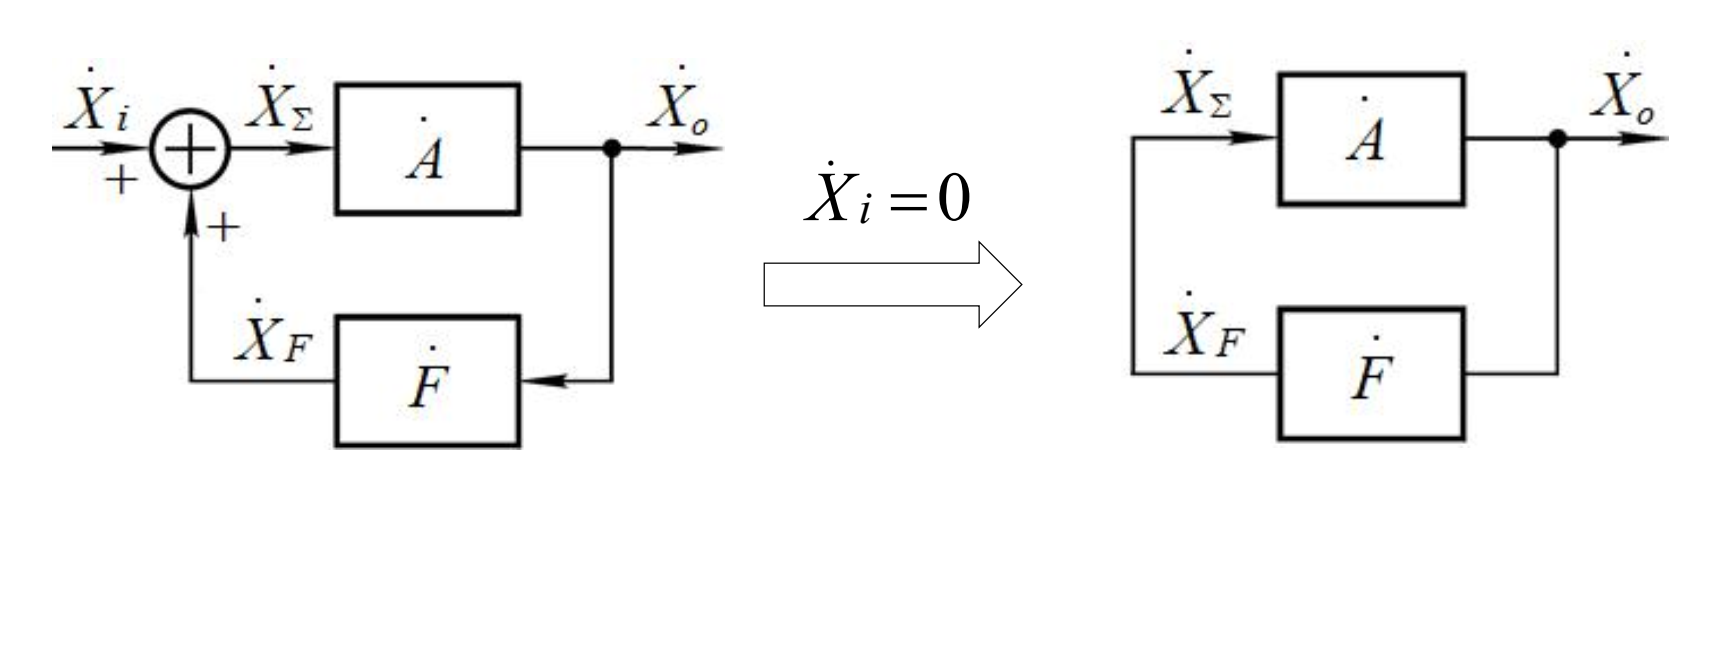
\includegraphics[width = \textwidth]{振荡原理1.png}

依照振荡器的特性,我们可以把它分为正弦波、 非正弦波振荡器与反馈型、 负阻型振荡器两大类。

当振荡器处于工作状态时,对其施加一个扰动信号(如信道噪声等),由于振荡器的AF大于1,外界噪声经历放大、选频等操作后,达到动态平衡,最终实现平衡。工作信号的变化如图2所示
\begin{center}
	
	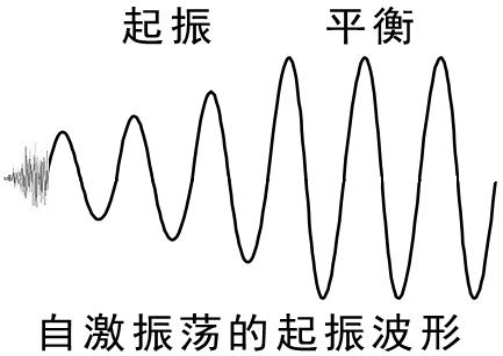
\includegraphics[width = 0.45\textwidth]{波形.png}
\end{center}
因此根据震荡器的工作原理,其应该在信号的初始阶段达成信号的放大,起振条件要求:
$$
\left\{\begin{array}{l}
	\text { 振幅起振条件 }|\dot{A} \dot{F}|>1 \\
	\text { 相位起振条件 } \phi_{A}+\phi_{F}=2 n \pi
\end{array}\right.
$$

而其达到动态平衡要求,输出幅度均匀的信号要求 $\dot{A} \dot{F}=1$, 包括振幅条件与相位条件两项
$$
\left\{\begin{array}{l}
	\text { 振幅平衡条件 }|\dot{A} \dot{F}|=1 \\
	\text { 相位平衡条件 } \phi_{A}+\phi_{F}=2 n \pi
\end{array}\right.
$$
我们将在实验中验证上述的起振条件和平衡要求

对于震荡发生器,其还应满足
振幅稳定条件: $\frac{\partial A}{\partial V_{o m}}<0$与相位稳定条件: $\frac{\partial \varphi}{\partial \omega}<0$


本次实验中,以上两个条件振荡器自动满足,我们不考虑。



实验所用文氏电路板设计如图。文氏电桥包含一个放大电路和一个正反馈网络。放大电路
为三极管 3DG6 构成的两级共射电路,而正反馈网络则由 (C1; R1; R2) 构成,由于正反馈网络由 RC
元件构成,其频率响应使得正反馈网络兼有选频作用

	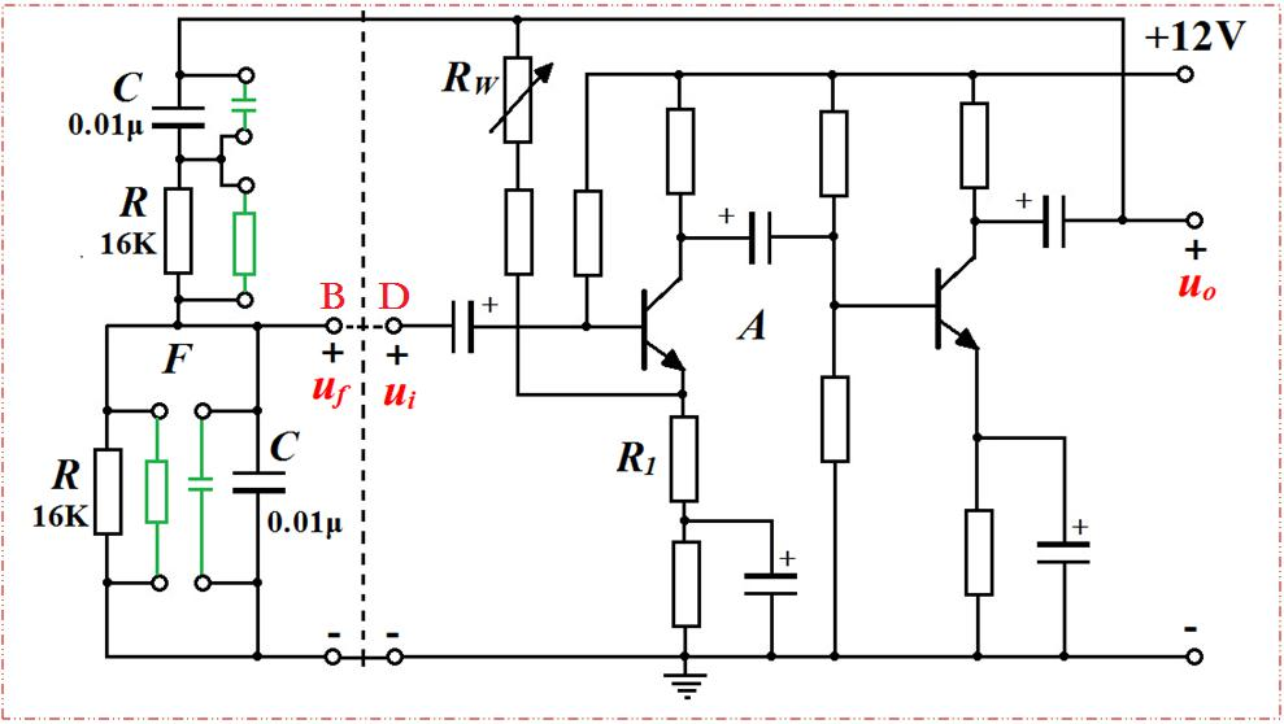
\includegraphics[width = \textwidth]{实验电路图.png}


\begin{center}
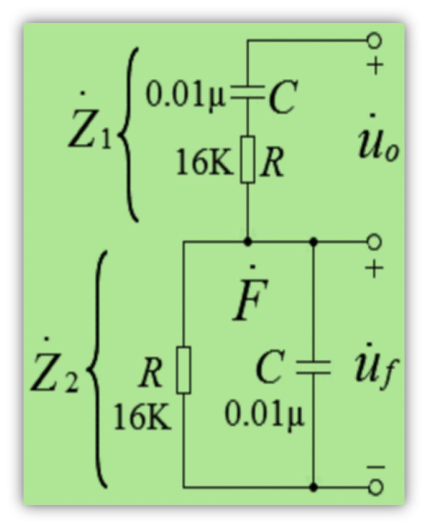
\includegraphics[width=0.3\textwidth]{反馈网络.png}
\end{center}
其对应的反馈网络如图

理论计算告诉我们,反馈网络的相关参数计算如下
$$
\dot{Z}_{1}=R+\frac{1}{j \omega C} ; \quad \dot{Z}_{2}=R / / \frac{1}{j \omega C}
$$
$$
\dot{F}=\frac{\dot{u}_{f}}{\dot{u}_{o}}=\frac{\dot{Z}_{2}}{\dot{Z}_{1}+\dot{Z}_{2}}=\frac{1}{3+j\left(\omega R C-\frac{1}{\omega R C}\right)}
$$

通过理论计算我们可以大致分析该振荡器的放大倍数与工作模式。振荡器中的文氏电桥选频网络在不同频率时的响应不同,输入输出间的幅度与相位均与频率有关。
在输入频率增加时,输出信号 Vf 与输入信号 Vs 的相位差不断变化,从接近 −90◦ 不断增至 90◦,在某个频率 f0 处取 0。幅度比先增大,在中心频率 f0 处取得极大值,后不断减小,这样在中心频率处
同时满足幅度与相位条件,发挥选频作用

我们将在实验部分进一步对理论预言结果进行验证。




\section{实验内容与步骤}
\subsection{测量振荡器的振荡幅度 $V_{0}$}
(1) $\mathrm{R}=16 \mathrm{~K} \Omega, \mathrm{C}=0.01 \mu \mathrm{F}$, 振荡器接 $+12 V$ 电源、连 接 $B 、 D$ 两点, 振荡器输出端接示波器;


(2)调节振荡器中 $\boldsymbol{R}_{W}$, 使振荡器输出不失真正弦波, 测量输出电压幅值(cursors法、meas法、万 用表 $\mathbf{A C V}$ 法)。

\subsection{测量振荡器的震荡频率$f_0$}
1、示波器测量 $f_{0}$ ( cursors法、meas法)

2、李莎育图形法测量$f_{0}$

(1) 调节振荡器中 $\boldsymbol{R}_{\boldsymbol{}}$, 使振荡器输出不失真正弦波。


(2) 示波器 1 通道接信号源, 示波器 2 通道接振荡器, 示波器 设置为【 X-Y 】工作模式 (Horiz $\rightarrow$ 时基模式 $\rightarrow \mathbf{X}-\mathbf{Y}$ ) 。


(3) 调节信号源频率 $\boldsymbol{f}_{\boldsymbol{i}}$ 出现如下稳定图形之一, 计算振荡 频率 $\boldsymbol{f}_{\mathbf{0}}$ 。

\begin{figure}
	\centering
	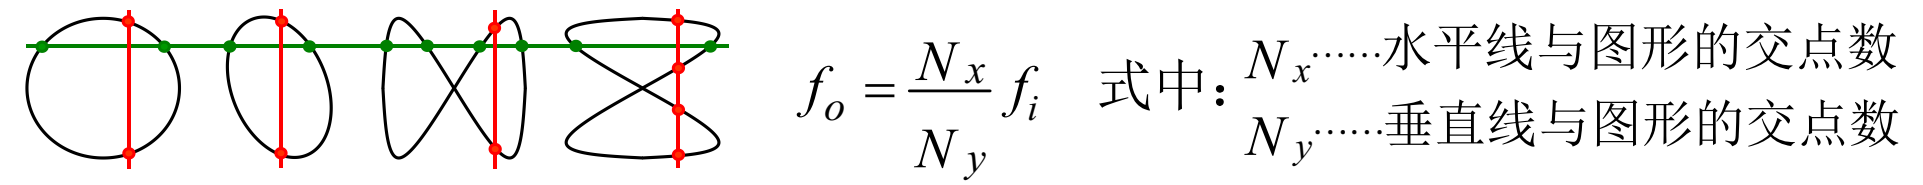
\includegraphics[width = \textwidth]{李萨如正式.png}
\end{figure}


\subparagraph{测量频率稳定度}
(1) 一定时间内: $\frac{\Delta f}{f_{o}}=\frac{\left|f_{o x}-f_{o}\right|}{f_{o}} \quad \begin{aligned}&f_{o x} \cdots \cdots \text { 为最大偏离值 } \\&f_{o} \cdots \cdots \text { 多次测量平均估 }\end{aligned}$ 

(2) $\mathbf{E}_{\mathbf{C}}$ 变化: $\frac{\Delta f}{f_{o}}=\frac{\left|f_{o x}-f_{o}\right|}{f_{o}} \quad \begin{aligned}&f_{o x} \cdots \cdots E_{c}=10 \mathrm{~V} \text { 测量数据 } \\&f_{o} \cdots \cdots E_{c}=12 \mathrm{~V} \text { 测量数据 }\end{aligned}$

\subparagraph{测试振荡器的三种工作状态}

状态 1:


(1) 连接 $u_{f}$ (B)与 $u_{i}$ (D)两点, 调节 $R_{W}$ 使振荡器输出不失真正弦波形。 

(2) 断开 $u_{f}$ 与 $u_{i}$ 两点, 从 $u_{i}$ 点接入频率为 $f_{o}$ 的正弦信号, 选择合适的 $u_{i}$ 幅值使 $u_{o}$ 不失真, 用数字电压表 $\mathrm{ACV}$ 功能测量 $u_{i} 、 u_{o}$ 及 $u_{f}$, 计算放大器的电压放大 倍数 $A=u_{o} / u_{i}$ 和环路增益 $F A$ 。


状态 $2:$


断开 $u_{i}$ 信号, 连接 $u_{f}$ 与 $u_{i}$ 两点, 调节 $R_{W}$ 使振荡器输出失真波形, 重复(2)。 

状态3:


断开 $u_{i}$ 信号, 连接 $u_{f}$ 与 $u_{i}$ 两点, 调节 $R_{W}$ 使振荡器停振, 重复(2)。

\subparagraph{ 观察起振与停振过程}

(1) 扫描速率 $T / D I V \approx 100 m s$ 。


(2) 缓慢调节 $\boldsymbol{R}_{\mathbf{W}}$, 观察起振与停振过程。


(3) 记录起振与停振过程图。

\subparagraph{测量RC串并联网络的幅频特性和相频特性}

(1) 将RC串并联网络的输出端 $u_{f}$ 与放大器的输入端 $u_{i}$ 断开。


(2) 信号源输出接放大器输入 $u_{i}(0.5 \mathrm{Vpp})$, 示波器 1 通道接 放大器输出 $u_{0}$ 端, 2 通道接 $\mathrm{RC}$ 网络输出 $u_{f}$ 端。


(3) 选取不同的信号频率 $f$, 测量 $u_{0}$ (不失真) 和 $u_{f}$ 以及它们 之间的相移 $\pm \theta^{0}$, 计算反馈系数 $F=\frac{u_{f}}{u_{o}}$
找出使 $F$ 值最大的频率点及对应 $0.707 F$ 的频率点。








\section{实验数据处理与分析}

\subsection{测量振荡器的振荡幅度}
	连接振荡器到12V直流电源,调整示波器波形为不失真,通过三种方法得到测量的电压值于表一
	% Table generated by Excel2LaTeX from sheet 'Sheet1'
	\begin{table}[htbp]
		\centering
		\caption{ 不同方式测量振荡器输出幅度数据记录}
		\begin{tabular}{ll}
			测量方法  & 结果 \\
			cursor法 & 6.16V(峰峰值) \\
			meas法 & 6.08V(峰峰值) \\
			ACV法  & 2.1419V(有效值) \\
		\end{tabular}%
		\label{tab:addlabel}%
	\end{table}%

	我们计算得到三种方法的输出平均值为
	\[V = \frac{2.1419+\frac{6.08}{2\sqrt{2}}+\frac{6.16}{2\sqrt{2}}}{3} = 2.1564\]
	几种结果的相对误差为
	\[\eta_1 = \frac{|\frac{6.16}{2\sqrt{2}}-2.1564|}{2.1564} = 0.00997\]
	\[\eta_2 = \frac{|\frac{6.08}{2\sqrt{2}}-2.1564|}{2.1564} = 0.00315\]
	\[\eta_3 = \frac{|2.1419-2.1564|}{2.1564} = 0.00672\]
	
	可能的误差来源包括仪器性能特点与实验者本身,光标法 (cursor 法) 的误差最大,最
	为准确的测量方法是用meas挡进行测量。我们分析得到,光标法因为涉及人为的读数操作以及示波器光标的最小分度值,估读误差较大,在有限次的测量中结果较为不准确。
	

	
	
	

\subsection{测量振荡频率}
	连接振荡器到12V直流电源,调整示波器波形为不失真,通过三种方法得到测量的频率值于表二
	% Table generated by Excel2LaTeX from sheet 'Sheet1'
	\begin{table}[htbp]
		\centering
		\caption{信号频率测量数据记录}
		\begin{tabular}{lr}
			测量方法  & \multicolumn{1}{l}{结果(HZ)} \\
			cursor法 & 954.2 \\
			meas法 & 954 \\
			万用表频率挡 & 955.88 \\
			李沙育图形法 & 956 \\
		\end{tabular}%
		\label{tab:addlabel}%
	\end{table}%
	对于李莎育图形法,调节 Rw 产生不失真正弦波后用示波器 CH1 接通信号源,示波器 CH2 接通振荡器,示波器设置为 X-Y 工作模式。当参考频率调节为 f =956.00Hz 时,得到了相对稳定的椭
	圆环形李莎育图形,可以看到此时实际频率与参考频率之间的比值为 1:1,因此可知实际频率
	fL = f = 956.00Hz。
	李沙育图形如图
	
	
	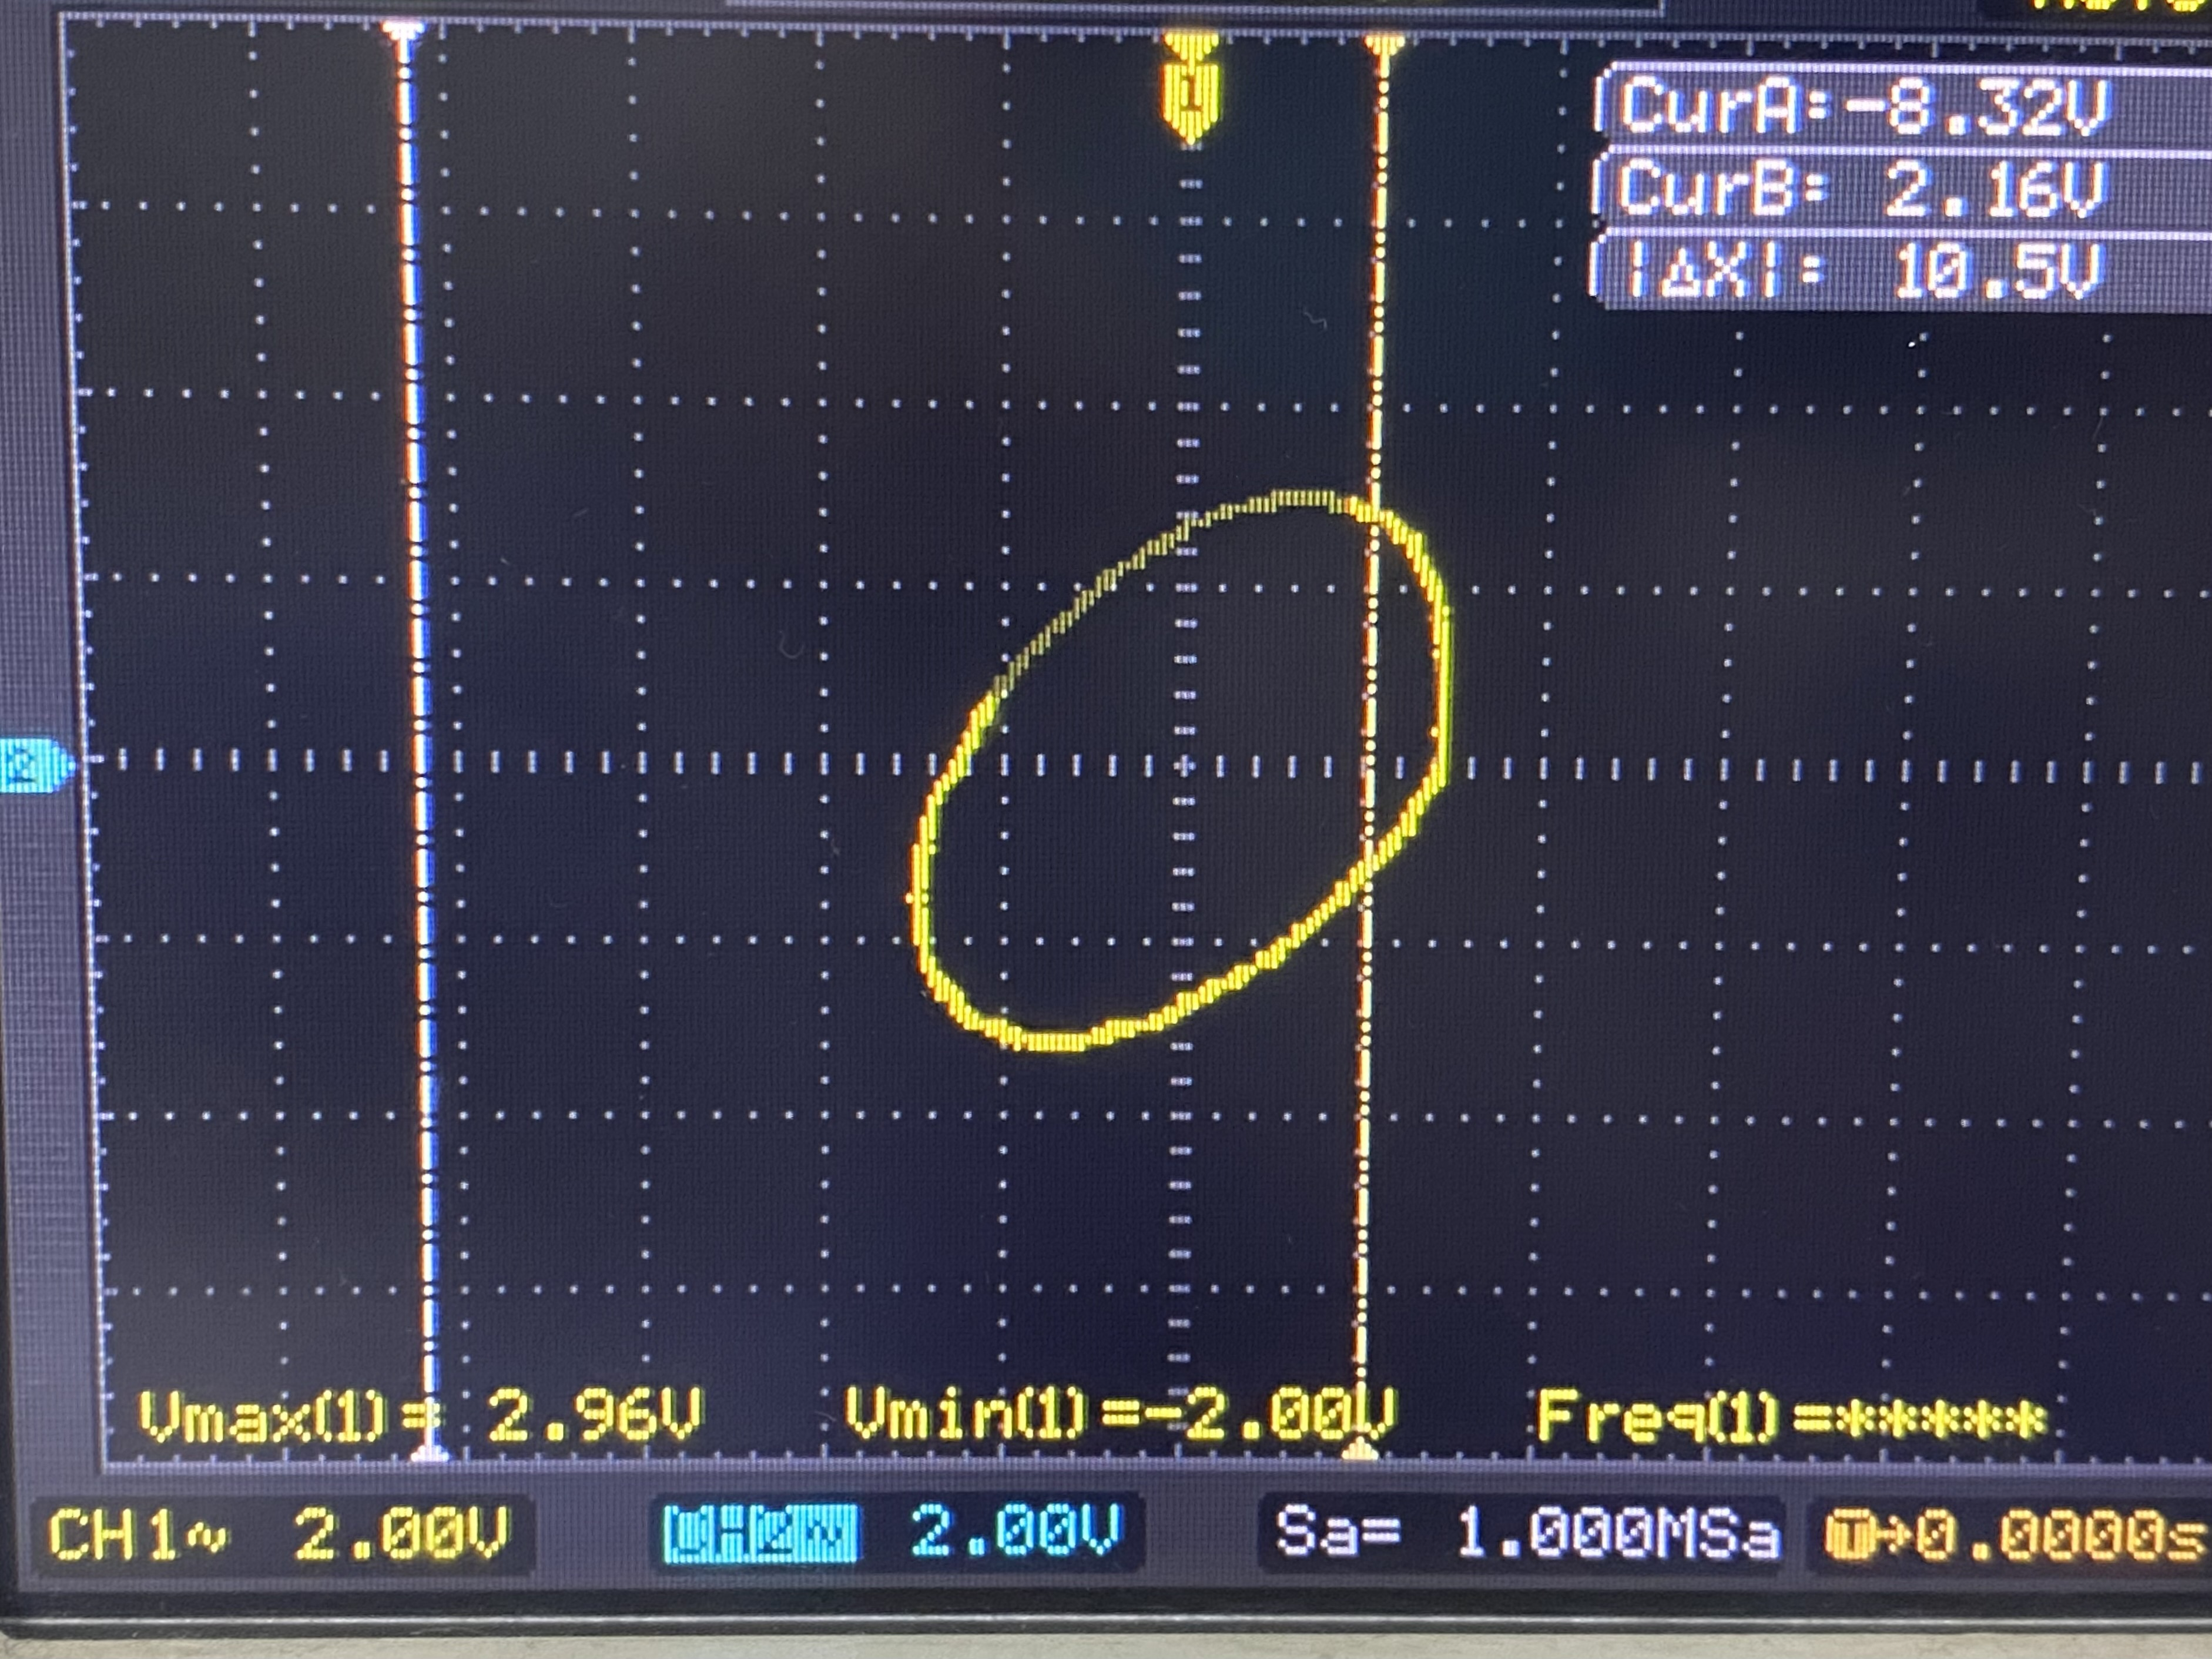
\includegraphics[width = \textwidth]{李萨如2.jpg}
	
	
	
	误差分析中,可以看到四次测量结果与平均值都十分接近,误差都相对较小
。
	
	
	另外通过观察李莎育图形的形态,即使在频率调定、李莎育图形固定后,也可见李莎育图形只能
	稳定较短的一段时间,在 30 秒后基本上就可见明显李莎育图形的旋转、扭动。这可能是因为振荡器的
	频率稳定性较差,导致其与信号源输出间不能长期维持稳定的相位差所致,也可能与信号源基准频率
	稳定度有限有关,还可能与手动设置信号源频率时判断李莎育图形稳定有一定的主观性有关。

	
\subsection{测量频率稳定度}

由于实验室环境难以控制,所以对温度、湿度等环境指标对频率的影响的测量比较困难。因此认
为这些量随时间浮动,体现为一个时变的“噪声”,并且对不同时间的测量能够表现这种不稳定性。


实验中在五分钟内多次对频率进行测量,测量方法使用数字万用表 Freq 挡直接测量。得到结果如
表三。

% Table generated by Excel2LaTeX from sheet 'Sheet1'
\begin{table}[htbp]
	\centering
	\caption{频率稳定性测量数据记录}
	\begin{tabular}{lrrrrrr}
		f/Hz  & 955.88 & 955.94 & 955.97 & 956.03 & 956.06 & 956.02 \\
		t/s   & 0     & 30    & 60    & 90    & 120   & 150 \\
		&       &       &       &       &       &  \\
		f/Hz  & 956.06 & 956.11 & 956.1 & 956.09 & 956.02 &  \\
		t/s   & 180   & 210   & 240   & 270   & 300   &  \\
	\end{tabular}%
	\label{tab:addlabel}%
\end{table}%

最大偏离值在$t = 210s$时取得,稳定度为
\[\frac{\Delta f}{f_0} = \frac{0.23}{955.88} = 0.00024\]


另外,直流供电电压也会对频率稳定性造成影响。当电源接入10V电压时,测得频率为$f = 955.16Hz$,可计算供电电压下降 2V 时频率稳定度为
\[\frac{\Delta f}{f_0} = \frac{0.72}{955.88} = 0.000753\]

可以看到,在本实验室环境下,环境因素导致的频率在随时间涨落在 0.0001 量级,对于
RC 稳频的简易振荡电路来说并不大。因此,我们说我们的RC振荡器具有较好的稳定性,可以提供较为稳定的正弦波电压

\subsection{测量三种工作状态}
振荡器一般有三种工作状态:保真工作状态、失真工作状态、停振工作状态。在不同的工作状态
下,放大网络增益 A 与开环增益 F A 的数值不同,理论上在正常工作时,振荡器参数应满足振荡条
件2,在失真振荡时 F A > 1,当停振时应有 F A < 1。


实验中观察了不同振荡器运行状态下的增益 A 与开环增益 F A,数据见表四

% Table generated by Excel2LaTeX from sheet 'Sheet1'
\begin{table}[htbp]
	\centering
	\caption{不同振荡器运行状态下参数测量记录}
	\begin{tabular}{lrrrrr}
		& \multicolumn{1}{l}{U\_i/V} & \multicolumn{1}{l}{U\_i/V} & \multicolumn{1}{l}{U\_i/V} & \multicolumn{1}{l}{A} & \multicolumn{1}{l}{AF} \\
		保真    & 0.37826 & 1.1564 & 0.3741 & 3.0572 & 0.989 \\
		失真    & 0.37827 & 1.7479 & 0.58536 & 4.6208 & 1.5475 \\
		停振    & 0.37824 & 0.92589 & 0.31015 & 2.4479 & 0.81998 \\
	\end{tabular}%
	\label{tab:addlabel}%
\end{table}%

由此可见,当桥式电路处于保真工作状态时,其放大器增益 A = 3.0572 接近 3,开环增
益 F A = 0.989 接近于 1,与理论预期相符合;而失真振荡时 A = 4.6208 大于 3,F A = 1.5475 大于 1;
当停振时,A = 2.4479 小于 3,F A = 0.81998 值明显地小于 1。这些结果都与振荡条件理论相符合。


\subsection{观察起振与停振}
用示波器观察缓慢调节电位器 Rw 时的起振与停振过程,记录得起振过程如图。

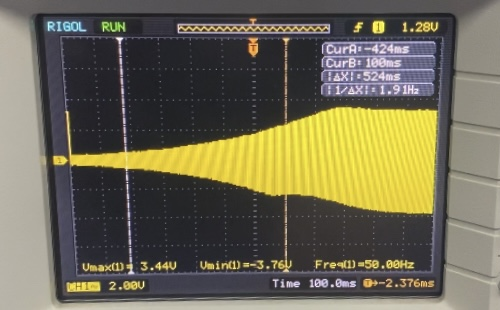
\includegraphics[width = \textwidth]{起振.png}

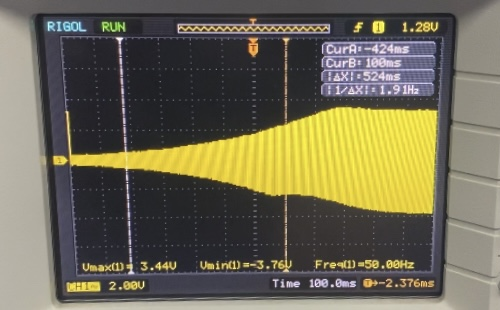
\includegraphics[width = \textwidth]{停摆.png}



\subsection{幅频特性与相频特性}
测量得到振荡器电路的幅频特性与相频特性如表四
% Table generated by Excel2LaTeX from sheet 'Sheet1'
\begin{table}[htbp]
	\centering
	\caption{Add caption}
	\begin{tabular}{lrrrrrrrr}
		f/Hz  & 100   & 300   & 500   & 700   & 900   & 1000  & 1100  & 1200 \\
		$U_0$/V & 1.3315 & 1.3322 & 1.331 & 1.3301 & 1.3293 & 1.3289 & 1.3287 & 1.3281 \\
		$U_f$/V & 0.13642 & 0.33261 & 0.40329 & 0.4331 & 0.44112 & 0.4409 & 0.43878 & 0.43521 \\
		$\theta$/° & -70   & -43   & -25   & -12   & -2    & 1     & 6     & 9 \\
		F$\times 10^-3$     & 102.46 & 242.16 & 302.99 & 325.39 & 331.9 & 331.78 & 330.23 & 327.69 \\
		&       &       &       &       &       &       &       &  \\
		f/Hz  & 1300  & 1400  & 1600  & 1800  & 2000  & 3000  & 3230  &  \\
		$U_0$/V & 1.3276 & 1.3272 & 1.3264 & 1.3259 & 1.3254 & 1.3231 & 1.3221 &  \\
		$U_f$/V & 0.43063 & 0.42532 & 0.41311 & 0.39953 & 0.3856 & 0.318 & 0.30914 &  \\
		$\theta$/° & 11    & 14    & 18    & 25    & 28    & 42    & 46    &  \\
		F$\times 10^-3$     & 324.37 & 320.46 & 311.45 & 301.33 & 290.93 & 240.34 & 233.82 &  \\
	\end{tabular}%
	\label{tab:addlabel}%
\end{table}%
从表中我们可以得到对应0.707F的频率值约为300Hz与3230Hz,为振荡器的上下截止频率。因此本桥式振荡电路
选频网络的带宽 BW=3230-300=2930Hz。其带宽较宽,选频特性并不佳。





\section{实验总结}
在本次实验中,我们利用示波器搭建与测量了RC一阶电路的响应电路、微分和积分电路以及脉冲分压电路
虽然有一定的误差,但在实验设计允许范围内,和理论吻合得较好,成果较为令人满意。通过这次实验也学习到了
一阶电路的一些特性,熟悉了时间常数有关的概念,锻炼了实验能力和误差分析能力。
\newpage

\section{思考题}
问 1: 分析出现三种工作状态的原因。


答: 出现三种不同工作状态是由于在振荡限幅控制电位器 $R_{w}$ 取值不同时, 放大部分增益 $A$ 与限 幅值不同, 此时的振荡器开环增益 $A F$ 不同, 在某些时候在中心频率附近 $A F$ 乘积绝对值恰好等于 1 , 电路可维持稳定不失真振荡; 在某些时候 $A$ 小于 3 , 中心频率附近因为文氏电桥特性, $F<1 / 3, A F$ 乘积绝对值仍然小于 1 , 无法在任一频点上达到起振条件或振荡条件(吕), (2), 所以电路不能起振或振荡 在很短的时间内衰减, 进入停振状态。而在某些 $R_{w}$ 的取值下 $|A|$ 大于 1 , 使得其他频率处 $A F$ 仍然 可能大于 1 , 允许激发出谐波等其他频率信号, 造成失真工作状态。
\\

问 2 : 如果本实验电路中的放大器改用单级共射放大器, 请分析电路的工作状态。


答: 单级共射放大器的输出信号与输入信号相位相反, 在不另加移相部分或改变文氏电桥接法为 移相网络时来补偿这个 $\pi$ 的相位差时, 无法满足相位平衡条件, 不能起振。同时单级放大器的增益也 较低, 有一定可能不能满足振幅条件。
\\


问 3 : 设计一个振荡频率为 $30 \mathrm{kHz}$ 的 $\mathrm{RC}$ 文氏电桥振荡器。


答: 在设计中令选频网络中的 $R_{1}=R_{2}=R, C_{1}=C_{2}=C$, 则谐振频率满足公式
$$f=\frac{1}{2 \pi R C}$$


此时若选取 $R=1.608 \mathrm{k} \Omega, C=3.3 \mathrm{nF}$ 则可得到振荡频率为 $30 \mathrm{kHz}$ 的 $\mathrm{RC}$ 文氏电桥振荡器。
\\


\end{document}